\section*{Problem Sheet 4}
\label{sec:ps4}
\newcounter{psFourQuestions4}
\setcounter{psFourQuestions4}{0}
\renewcommand{\NewQuestion}[1]{\stepcounter{psFourQuestions4}\subsection*{Exercise \arabic{psFourQuestions4}: #1}}

\NewQuestion{CP-violation in \prt{B^{-} \to D\pi^{-}}}
\begin{enumerate}[a)]
\item Draw the tree-level Feynman diagrams for the decay \prt{B^- \to
    D^0 \pi^-} and \prt{B^- \to \overline{D}^0 \pi^-}.
  \answerbox{\\
    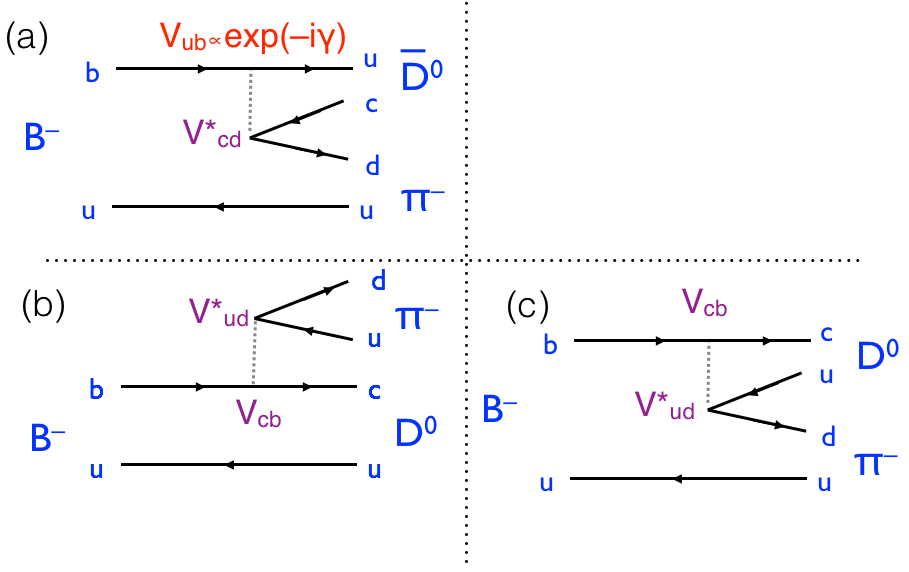
\includegraphics[width=0.9\textwidth]{problemsheets/ps4figs/B2DpiDiagrams}
  }
\item Consider the following final states $f$ of the D from the
  \prt{B^- \to D^0\pi^-} decay: \prt{\pim \pip}, \prt{\Km \Kp},
  \prt{\Kp \pim}, \prt{\Km \pip}.  For each of these, calculate the
  CP-violating decay rate asymmetry between \prt{B^- \to D \pi^-},
  \prt{D \to \mathit{f}}, and the CP-conjugate decay \prt{B^+ \to D
    \pi^+}, \prt{D \to \mathit{\overline{f}}}. As previously, if you
  find that there is an amplitude that can be mediated by both a
  colour favoured and a colour favoured diagram (with the same vertex
  factors), you can, for simplicity, ignore the colour-suppressed
  diagram.
  \answerbox{
    \begin{itemize}
    \item  Diagrams (a) and (c) are colour suppressed, while (b) is
      colour-allowed, so, for this
      calculation, we'll ignore (c). 
    \item Let us now calculate the ratio of amplitudes $
      \frac{A(\prt{B^- \to \Dob \pi^-})}{A(\prt{B^- \to \Do \pi^-})}$,
      that we'll call $r_B^{D\pi} e^{i\phi_{D\pi}}$ (you can of course call it
      what you like).
      \[
      r_B^{D\pi} e^{i\phi_{D\pi}} = \frac{A(\prt{B^- \to \Dob \pi^-})}{A(\prt{B^- \to \Do \pi^-})}
      \]
      To do so, we follow the same logic as in question 1 of problems sheet
      2. $A(\prt{B^- \to \Dob \pi^-})$ is proportional to the product of
      CKM matrix elements $V_{ub} V_{cd}^*$, multiplied by $1/\sqrt{3}$ to
      account for the colour suppression of diagram (a). $A(\prt{B^- \to
        \Do \pi^-})$ is proportional to $V_{ud}^* V_{cb}$. Hence
      \[
      r_B^{D\pi} e^{i\phi_{D\pi}} = 
      \frac{A(\prt{B^- \to \Dob \pi^-})}{A(\prt{B^- \to \Do \pi^-})} = 
      \frac{V_{ub} \cdot V^*_{cd}}{\sqrt{3} \; V_{cb} \cdot V_{ud}^*} e^{i\delta_B^{D\pi}}
      \]
      where we put in the ``ad hoc'' factor $e^{i\delta_B^{D\pi}}$ to take into
      account the phase difference between $A(\prt{B^- \to \Dob \pi^-})$
      and $A(\prt{B^- \to \Do \pi^-})$, that we cannot derive
      from the diagrams above, which only take into account the weak
      interaction, but that is nevertheless there.
      From the formula sheet: 
      \begin{itemize}
      \item $V_{ub}   = 0.0037 \cdot e^{-i\gamma}$
      \item $V_{cd}^* = -0.23$
      \item $V_{cb}   = 0.041$
      \item $V_{ud}^* = 0.97$
      \end{itemize}
      Hence
      \[
      r_B^{D\pi} e^{i\phi_{D\pi}} \approx -0.012 e^{i(\delta_B^{D\pi} -
        \gamma)}
      = 0.012 e^{i(\delta_B^{D\pi} + \pi - \gamma)}
      \]
    \item We are asked to calculate the rate asymmetry for four
      different final states of the \Do. Let's start with \prt{B^- \to
        (\Kp\pim)_D \pi^-}.  To calculate the full thing it is useful to
      draw the following diagram of the interfering amplitudes:
      \\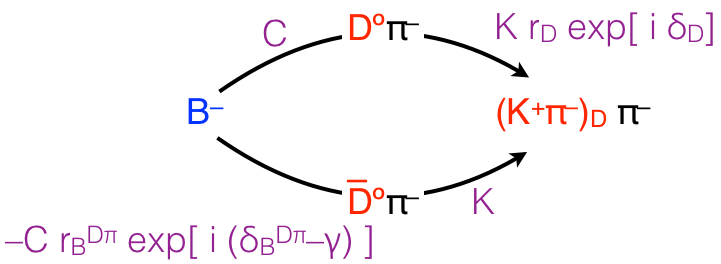
\includegraphics[width=0.6\textwidth]{problemsheets/ps4figs/B2Dpi_Interference}\\
      We'll need to estimate the ratio of amplitudes $\frac{A(\prt{\Do \to
          K^+ \pi^-})}{A(\prt{\Dob\to K^+\pi^-})}$. The relevant diagrams
      are
      \\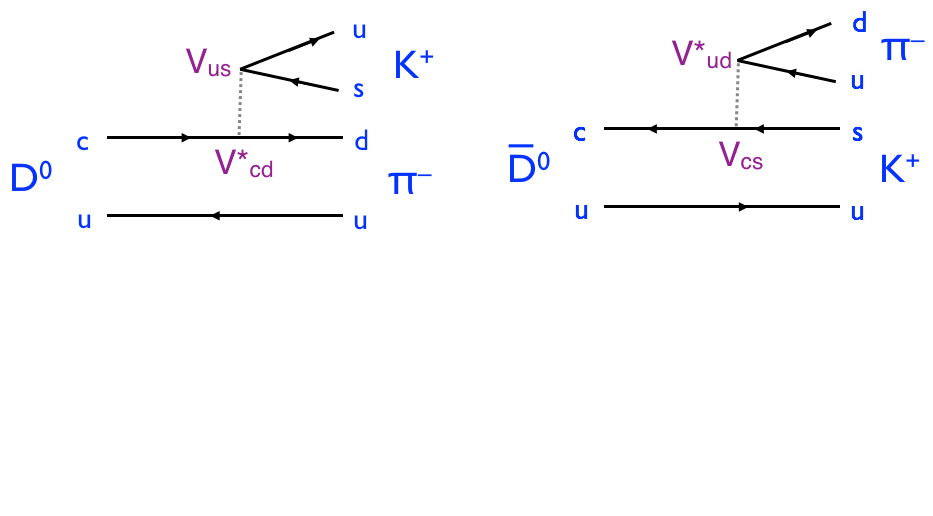
\includegraphics[width=0.65\textwidth]{problemsheets/ps2figs/D2KpiDiagrams}.\\
      The ratio of the \Do\ decay amplitudes involved is:
      \[
      \frac{A(\prt{\Do \to K^+ \pi^-})}{A(\prt{\Dob\to
          K^+\pi^-})} e^{i\delta_D}
      =
      \frac{V_{cd}^* V_{us}}{ V_{ud}^* V_{cs}}
      \approx \cos^2(\theta_C) = 0.05 e^{i\delta_D}
      \]
      where $\delta_D$ is again due to the strong interaction. We'll call
      the magnitude of this ratio $r_D$. We also introduce the complex
      factor $C$ and $K$ as $C \equiv A(\prt{B^- \to \Do \pi^-})$ and $K
      \equiv A(\prt{\Dob\to K^+\pi^-})$.
      Let's now calculate the rate $\Gamma(B^- \to (\Kp \pim)_D \pi^-)$:
      \begin{eqnarray*}
        \Gamma(B^-) & = & 
        \left| CK r_D^{K\pi} e^{i\delta_D^{K\pi}} + CK r_B^{D\pi} e^{i(-\gamma + \delta_B)} \right|^2
        \\ & = &
        C^2 K^2 \left({r_D^{K\pi}}^2 + (r_B^{D\pi})^2 {\color{red}+} 2r_D^{K\pi}\,r_B^{D\pi}\,\cos\left(-\gamma +\delta_B^{D\pi}-\delta_D^{K\pi} \right)\right)
        \\ & = & C^2K^2\left({r_D^{K\pi}}^2 + (r_B^{D\pi})^2 {\color{red}+} 2r_D^{K\pi}\,r_B^{D\pi}\, \left(
            \cos(\delta_B^{D\pi}-\delta_D^{K\pi})\,\cos\gamma -
            \sin(\delta_B^{D\pi}-\delta_D^{K\pi})\,\sin\gamma\right)\right)
      \end{eqnarray*}
      Next thing we need to calculate is the \cp-conjugate rate,
      $\Gamma(B^+ \to (\Km \pip)_D \pi^+)$.
      This is easy, given we have $\Gamma(B^- \to (\Kp \pim)_D \pi^-)$. We
      simply change the sign of the weak (CKM) phases (here, only $\gamma$):
      \begin{eqnarray*}
        \Gamma(B^+) & = & 
        C^2K^2\left({r_D^{K\pi}}^2 + (r_B^{D\pi})^2 - 2r_D^{K\pi}\,r_B^{D\pi}\, \left(
            \cos(\delta_B^{D\pi}-\delta_D^{K\pi})\,\cos\gamma +
            \sin(\delta_B^{D\pi}-\delta_D^{K\pi})\,\sin\gamma\right)\right)
      \end{eqnarray*}
      The decay rate asymmetry is:
      \begin{eqnarray*}
        A_{CP}^{\Kp\pim} & = & 
        \frac{
          {\color{red}+}2r_D^{K\pi}\,r_B^{D\pi}\,\sin(\delta_B-\delta_D^{K\pi})\,\sin\gamma
        }{
          {r_D^{K\pi}}^2 + (r_B^{D\pi})^2 + 2r_D^{K\pi}\,r_B^{D\pi}\, \cos(\delta_B^{D\pi}-\delta_D^{K\pi})\,\cos\gamma
        } 
        \\ & = & 
        \frac{
          -2\,\frac{r_B}{r_D^{K\pi}}\,\sin(\delta_B-\delta_D^{K\pi})\,\sin\gamma
        }{
          1 + \left(\frac{r_B}{r_D^{K\pi}}\right)^2 
          + 2\frac{r_B}{r_D^{K\pi}} \cos(\delta_B-\delta_D^{K\pi})\,\cos\gamma
        } 
        \\ & & \mbox{which is the same as}
        \\ & = & 
        \frac{
          -2\,\frac{r_D^{K\pi}}{r_B}\,\sin(\delta_B-\delta_D^{K\pi})\,\sin\gamma
        }{
          1 + \left(\frac{r_D^{K\pi}}{r_B}\right)^2 
          + 2\frac{r_D^{K\pi}}{r_B} \cos(\delta_B-\delta_D^{K\pi})\,\cos\gamma
        } 
      \end{eqnarray*}
  \item The other asymmetries are now quite easy to calculate. Let's
    start with the one for  $\Gamma(\prt{B^+ \to (\Kp \pim)_D
    \pi^+})$. We'll simply have to replace $r_D^{i\delta_D}$
    with $\frac{1}{r_D^{i\delta_D}} = \frac{1}{r_D} e^{-i\delta_D}$:
    \begin{eqnarray*}
      A_{CP}^{\Km\pip} & = &
      \frac{
        {\color{red}+}2\, r_B^{D\pi} r_D^{K\pi}\,\sin(\delta_B^{K\pi}+\delta_D^{K\pi})\,\sin\gamma
      }{
        1 + \left(r_B^{D\pi} r_D^{K\pi}\right)^2 
        + 2 r_B^{D\pi} r_D^{K\pi} \cos(\delta_B^{K\pi} + \delta_D^{K\pi})\,\cos\gamma
      } 
    \end{eqnarray*}
  \item For the asymmetries with \prt{D \to \Kp\Km} and \prt{D \to
      \pip\pim}, we replace $r_D^{i\delta_D}$ with 1.
    \begin{eqnarray*}
      A_{CP}^{KK} = A_{CP}^{\pi\pi} & = &
      \frac{
        {\color{red}+}2\, r_B^{D\pi} \,\sin(\delta_B)\,\sin\gamma
      }{
        1 + \left(r_B^{D\pi}\right)^2 
        + 2 r_B^{D\pi} \cos(\delta_B)\,\cos\gamma
      } 
    \end{eqnarray*}
  \item We've now answered the question as stated, but let's go one
    step further and estimate some numerical values. We don't
    know $\delta_B^{D\pi}$ or $\delta_D^{K\pi}$, but we know that 
    $|\sin(...)| \le 1$. Using this, the values for $r_B^{D\pi}$ and
    $r_D^{K\pi}$ we estimated, and $\gamma = 68^{\circ}$ we can
    estimate upper limits on the asymmetries:
    \begin{eqnarray*}
      A_{CP}^{\Kp\pim} & \le & \left|
        \frac{
          2\,\frac{r_B^{D\pi}}{r_D^{K\pi}} \sin\gamma
        }{
          1 + \left(\frac{r_B^{D\pi}}{r_D^{K\pi}}\right)^2 
        }\right|  = 0.42 \\
      A_{CP}^{\Km\pip} & \le & \left|
      \frac{
         2\, r_B^{D\pi} r_D^{K\pi}\,\sin\gamma
      }{
        1 + \left(r_B^{D\pi} r_D^{K\pi}\right)^2 
      }\right| = 0.0011
      \\
      A_{CP}^{KK} = A_{CP}^{\pi\pi} & \le &
      \left|\frac{
        2\, r_B^{D\pi} \,\sin\gamma
      }{
        1 + \left(r_B^{D\pi}\right)^2 
      }\right| = 0.022
    \end{eqnarray*}
    So we see that using a decay mode where the suppressed \prt{\Bpm
      \to D\pi^{\pm}} decay amplitude is matched by a favoured \Do\
    decay amplitude and vice versa maximises the asymmetry. Using the
    opposite theme, where the suppressed \Do\ decay amplitude and the
    suppressed \Bpm\ decay amplitude in the same decay path minimises
    the asymmetry. And using a \Do\ decay to a CP eigenstate like
    \prt{\Km\Kp}, where both decay amplitudes (\prt{\Do \to \Kp\Km}
    and \prt{\Do \to \Km \Kp}) are the same gives a result somewhere
    in the middle.
  \item One last note: as in the previous exercise, we somewhat
    over-estimated $r_B^{D\pi}$, but got qualitatively the right
    result. Had we taken into account the colour-suppressed diagram
    (c) that we ignored, we would have gotten closer to the truth. But
    the key missing element is the effect of the strong interaction,
    which we reduced to a factor $\frac{1}{\sqrt{3}} e^{i\delta_B}$,
    is much more complicated its effect is very difficult to calculate
    precisely, because the strong coupling constant $\alpha_S$ is so
    large at the energies we are dealing with, here, that the
    ``Taylor'' series expansion in terms of $\alpha$, which is at the
    basis of the Feynman diagram formalism, does not converge,
    depriving us of our favourite calculational method. In our
    calculation, we assumed that the effects of the strong interaction
    cancel in the decay rate ratio. This is not too far off, and good
    enough for an estimate like this, but it's simply not exactly true.
  \end{itemize}
}
\end{enumerate}
\NewQuestion{Higgs and BSM}
ATLAS and CMS have both seen hints of a new particle with a mass near
750GeV decaying to two photons. Some speculate that this might be a
"heavy Higgs", such as predicted by Super Symmetry and many other
Beyond the Standard Model (BSM) theories.
\begin{enumerate}[a)]
\item What motivates the search for physics beyond the Standard Model (SM)
  (List as many "flaws" of the SM as you know that indicate that the SM is
  not the final theory)?
  %% 
  \answerbox{
    There are a number or reasons why we are still not happy with the SM. They can be divided into two classes.
    \begin{enumerate}
    \item Real problems - discrepancies of the SM with reality.
    \item Aesthetic problems - aspects of the SM we find unsatisfactory (but not necessarily wrong)
    \end{enumerate}
    
    A problems of the first type include
    \begin{itemize}
    \item The baryon asymmetry of the universe: There is more matter (and more baryons) in the universe than anti-baryons. The SM does not provide a mechanism for generating this asymmetry for a matter-antimatter symmetric start.
    \item Dark matter: There is strong cosmological evidence fore dark matter, likely due to a fairly heavy, neutral particle. The SM does not provide a candidate for this. Many theories beyond the SM have a heavy, neutral, stable dark matter candidate.
    \item Gravity: simply missing
    \end{itemize}
    
    Problems of the second type include:
    \begin{itemize}
    \item The Hierarchy problem - there are in fact many hierarchy
      problems, but \emph{the} hierarchy problem is the difference in
      scale between the energy scale where the e/w forces unify
      (around the W and Higgs mass, i.e. $10^2$ GeV), compared to the
      mass where gravity becomes important, which $~10^{19}$GeV. This
      turns out to be the same question why gravity is soo much weaker
      than then the other forces.
    \item The fine tuning problem. This is closely related to the
      Hierarchy problem. "Naturally" one would expect the Higgs mass
      to be $~10^{19}$ in the SM. There are parameters in the SM that
      have to cancel to 11 digits in order to produce a Higgs mass
      with a "reasonable value" of $~10^2$ GeV. Such an exact
      cancellation, without any particular reason (such as a symmetry
      or so) is called fine tuning.
    \item There are other, less dramatic hierarchy problems. Why are
      the masses between the particles so different (neutrinos $<1eV$,
      top $>10^7 eV$)? In general it would be nice to have a model
      that \emph{predicts} the particle masses.
    \item The SM has too many free parameters (related to the previous
      point). The lepton masses, CKM parameters, PMNS parameters are
      all inputs to the theory, wouldn't it be nicer if they were
      outputs? Also, the structure seen in the mixing matrices suggest
      there should be some kind of underlying principle that explains
      them.
    \end{itemize}
  }
\item Assuming this particle really exists and that it has the same
  couplings (vertex factors) as the SM Higgs (but that, for some
  reason, it does not couple to the SM Higgs itself): What would be
  its preferred decay mode to SM particles?
  %% 
  \answerbox{It would predominantly decay to the heaviest particles
    that are kinematically allowed - so it would predominantly decay
    to $t\overline{t}$ pairs.}
\item Why is it difficult to see the SM Higgs, and this new
  particle, in their preferred decay modes at the LHC?
  %% 
  \answerbox{The top predominantly decays to a $b$ quark and a $W$
    (this is because $V_{tb}$ is much larger than other CKM
    elements related to the top). The $W$ can decay either to a pair
    of quarks, or to a lepton and a neutrino. So we see in our
    detector either
    \begin{itemize}
    \item a $b$ jet and two other jets
    \item a $b$ jet, a lepton (e.g. a $\mu$), and some missing momentum
    \end{itemize}
    Both is difficult (although not impossible) at the LHC. There are
    lots of jets at the LHC, including lots of b-jets (jets with
    b-quarks), produced in the proton-proton collisions. So we get a
    lot of background. The version with the lepton and the missing
    momentum is ``cleaner'', as there are not so many leptons produced
    in p-p collisions, but the missing momentum makes it impossible to
    reconstruct the mass precisely.  }
\end{enumerate}
\NewQuestion{Consider the decays}
\begin{enumerate}[i)]
\item \prt{B_s^0 \to \Kp\Km}
\item \prt{B_d^0 \to \pip\pim}
\end{enumerate}
(and their CP conjugates). 
\begin{enumerate}[a)]
\item Which combination of CKM phases can be probed with these decays?
Note: for the decay process, only consider
tree-level diagrams for your calculation (while of course the B-mixing
diagrams are loop diagrams, and they cannot be ignored).  
\answerbox{
  \begin{enumerate}[i)]
  \item The relevant diagrams are\\
    \begin{tabular}{cc}
      \Bso mixing & \prt{B_s^0 \to \Kp\Km} \\
      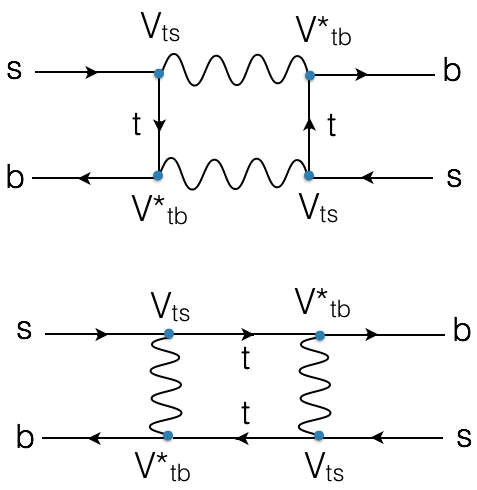
\includegraphics[width=0.3\textwidth]{problemsheets/ps4figs/BsMixingWithCKM}
      &
      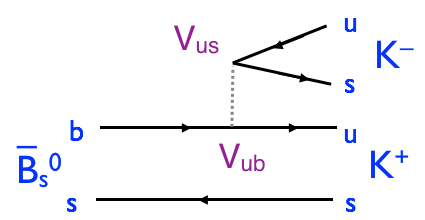
\includegraphics[width=0.3\textwidth]{problemsheets/ps4figs/Bs2KK}
      \\
      phase: $0$ & phase: $-\gamma$
    \end{tabular}\\
    Hence, the phases difference of the interfering amplitudes
    \\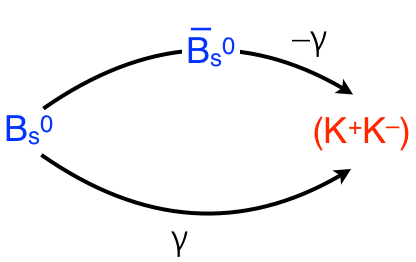
\includegraphics[width=0.35\textwidth]{problemsheets/ps4figs/Bs2KKInterference}
    \\
    is $2\gamma$ (so this is the phase we are sensitive to).
  \item The relevant diagrams are\\
    \begin{tabular}{cc}
      \Bdo mixing & \prt{\Bdob \to \pip\pim} \\
      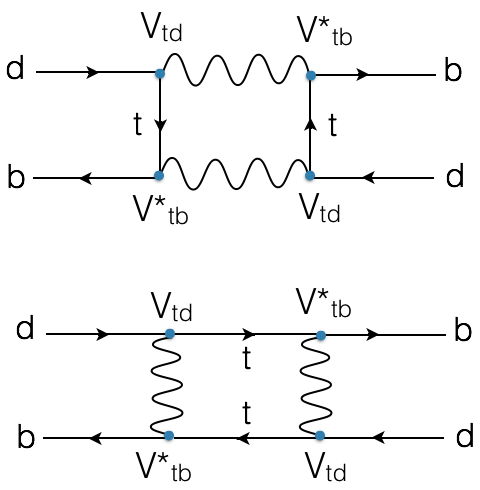
\includegraphics[width=0.3\textwidth]{problemsheets/ps4figs/BdMixingWithCKM}
      &
      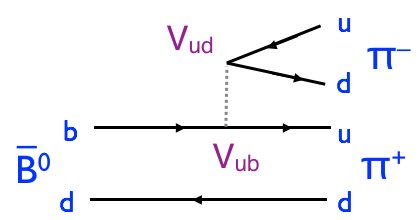
\includegraphics[width=0.3\textwidth]{problemsheets/ps4figs/Bd2pipi}
      \\
      phase: $-2\beta$ & phase: $-\gamma$
    \end{tabular}\\
    Hence, the phases difference of the interfering amplitudes
    \\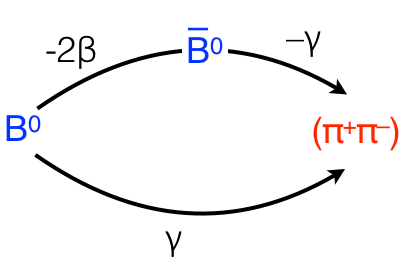
\includegraphics[width=0.35\textwidth]{problemsheets/ps4figs/B2pipiInterference}
    \\
    is $2(\beta + \gamma)$
  \end{enumerate}
}
\item If the CKM element $V_{ts}$ were not real (as in the formula sheet), but complex, $V_{ts} = -|V_{ts}|e^{-i\beta_s}$, which combination of phases would be measured, then?
\answerbox{\Bdo\ would remain the same, but the \Bso\ mixing diagram is proportional to $V_{ts}^2$, so the total phase difference between \prt{\Bso \to K^+ K^-} and \prt{\Bso \to \Bsob \to K^+ K^-} would be $- 2\beta_s -2\gamma$}
\item Draw the penguin diagrams for \prt{\Bdo \to \pi^+ \pi^-}\prt{\Bso \to K^+ K^-}. What are the (dominant) CKM phases in these diagrams?
\answerbox{
The diagram with an internal top quark line will dominate in each case, hence:\\
\begin{tabular}{ccc}
& 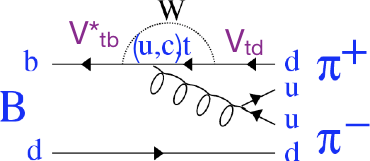
\includegraphics[width=0.4\textwidth]{fig/B2pipiPeng}
&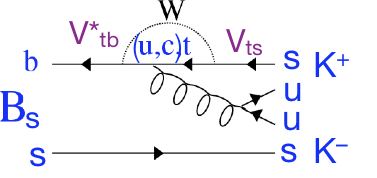
\includegraphics[width=0.4\textwidth]{problemsheets/ps4figs/Bs2KKpeng}\\
phase & $-2\beta$ & $-2\beta_s \approx 0$
\end{tabular}
(Remark: We could also have written for the \Bso\ decay mode that the phase is $-\beta + \pi$ because $V_{ts}$ as $V_{ts} = -|V_{ts}| e^{-i\beta_s} = |V_{ts}| e^{i(\pi -\beta_s)}$; however, this does not change whether a decay violates CP or not, nor what combination of CKM phases it is sensitive to, it's just a sign somewhere. So in an exam, at least as long you get the sign right in the rare cases where it matters, $-2\beta_s$ or $\pi - 2\beta_s$ would both have been an acceptable answer.)
}
\end{enumerate}
